\documentclass{beamer}

\usepackage{beamerthemesplit}
\usepackage{amsmath}
\usepackage{amsfonts}
\usepackage{amssymb}
\usepackage{qtree}
\usepackage{cancel}
\usepackage{tkz-graph}
\usepackage{bussproofs}
%\usepackage[pdftex]{graphicx}

\makeatletter
\newcommand{\reallytiny}{\@setfontsize{\srcsize}{2pt}{2pt}}
\makeatother

\mode<presentation>
{
  \usetheme{metropolis}
  % or ...

  %\setbeamercovered{transparent}
  % or whatever (possibly just delete it)
}

\usepackage[english]{babel}
% or whatever

\usepackage[latin1]{inputenc}
% or whatever

\usepackage{times}
\usepackage[T1]{fontenc}

\title{Inferential Approach to Mining Surprising Patterns in
  Hypergraphs}

\author{Nil Geisweiller, Ben Goertzel}

\institute[SingularityNET OpenCog Foundations] % (optional, but mostly needed)
{
  \begin{center}
    
\includegraphics[scale=0.5]{images/snet_oc.png}
  \end{center}
}

\date[AGI-19] % (optional, should be abbreviation of conference name)
{AGI-19, Shenzhen}

%\newcommand{\AND}{\textit{AND}}
%\newcommand{\OR}{\textit{OR}}
%\newcommand{\NOT}{\textit{NOT}}
\newcommand{\AND}{\land}
\newcommand{\OR}{\lor}
\newcommand{\NOT}{\lnot}

\begin{document}

\frame
{
%%%%%%%%%%%%
%% Speech %%
%%%%%%%%%%%%

%% This work starts with the motivation of reframing learning as an
%% explicit form of reasoning.

%% We claim that by doing that, reframing learning as reasoning you
%% gain more transparency and as a result you make it much easier to
%% enable meta-learning at all levels.

%% Here in particular we are gonna focus on mining suprising patterns.

%% All the work I'm gonna present here is implemented with the OpenCog
%% framework, and it is sponsored by SingularityNET.

%%%%%%%%%%%%%
%% ~Speech %%
%%%%%%%%%%%%%

  \maketitle
}

\begin{frame}
  \frametitle{Reframing \alert{learning as reasoning}}

%%%%%%%%%%%%
%% Speech %%
%%%%%%%%%%%%

%% OK, so what does reframing learning as reasoning mean?

%% What it means is, just think of any learning task, such as learning
%% how to recognize faces, which is translated as a task of proving a
%% certain theorem or a collection of theorems in a certain theory.

%%%%%%%%%%%%%
%% ~Speech %%
%%%%%%%%%%%%%

  \begin{columns}

    \column{2in}
    %% \begin{center}Learning\end{center}
    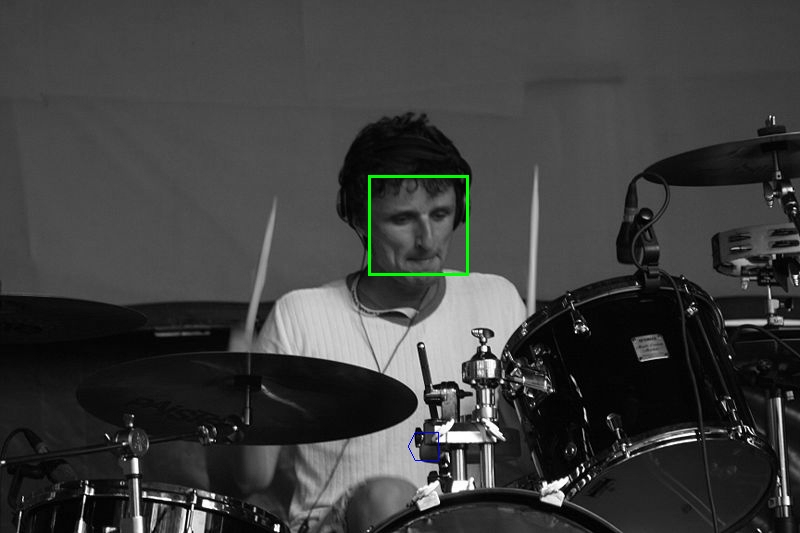
\includegraphics[scale=0.15]{images/800px-Cool_Kids_of_Death_Off_Festival_p_146-face_selected.jpg}

    \column{1in}
    $$ \Rightarrow $$

    \column{1in}
    %% \begin{center}Reasoning\end{center}
    $$ \mathcal{T} \vdash \mathcal{F} $$

  \end{columns}

\end{frame}

\begin{frame}
  \frametitle{Reframing \alert{mining surprising patterns as
      reasoning}}

%%%%%%%%%%%%
%% Speech %%
%%%%%%%%%%%%

%% More specifically we're gonna show how to do that for 2 problems

%% 1. the problem of finding frequent patterns in a database

%% 2. and the problem of assessing their surprisingness

%% To give you a broader picture. The reason we are interested in
%% these 2 problems, is because they are part of a greater
%% meta-learning scheme that I'm gonna present right now, that can be
%% called "Inference Control Meta-learning".

%%%%%%%%%%%%%
%% ~Speech %%
%%%%%%%%%%%%%

  \begin{enumerate}
  \item Learning \alert{frequent} patterns
  \item Assessing their \alert{surprisingness}
  \end{enumerate}

\end{frame}

\begin{frame}
  \frametitle{Inference Control Meta-learning}

%%%%%%%%%%%%
%% Speech %%
%%%%%%%%%%%%

%% As you probably already know the problem of reasoning is that it
%% rather inefficient in general, there is a combinatorial explosion
%% due to the number of rules and premises that can be chosen from to
%% build an inference. The complexity is basically growing exponential
%% with the size of the proof.

%% So it's important to be able to learn how to reason
%% efficiently. But once you reframe learning as reasoning, then it
%% becomes the problem of how to reason to reason efficiently, and
%% that creates a very direct feedback loop in your system.

%%%%%%%%%%%%%
%% ~Speech %%
%%%%%%%%%%%%%

  \begin{center}\alert{Learning how to reason efficiently}\end{center}
\end{frame}

\begin{frame}
  \frametitle{Inference Control Meta-learning}

%%%%%%%%%%%%
%% Speech %%
%%%%%%%%%%%%

%% I'm gonna present very briefly the system we have in place to do
%% that with opencog.

%% We have a rewriting system that we call the unified rule engine,
%% that can be used to implement any logical system, what is does is
%% that it that essentially evolves inference trees, given a theory
%% and a set of inference rules. it will build either in a forward
%% fashion, from premises to conclusions, from theory to theorems, or
%% in a backward fashion, from conclusions to premises, from theorems
%% to theory.

%% TODO  
  
%% Now the interesting thing about it is that it can use control rules
%% to decide how to select premises or conclusion and rules to
%% construct these inference trees, and so the idea is that if we can
%% learn the right control rules we can speed up reasoning. And that
%% is where pattern mining comes into place here, as a simple though
%% efficient way to kick start such feedback loop.

%% There is BTW another component of OpenCog called ECAN, that stands
%% for Economic Attention Allocation Networks, that is also designed
%% to speed up reasoning, that I'm letting aside here.

%%%%%%%%%%%%%
%% ~Speech %%
%%%%%%%%%%%%%

  Unified Rule Engine
  \begin{itemize}
  \item<+-> Evolves \alert{Inference Trees}
  \item<+-> \alert{Control Rules} to select premises and rules
  \end{itemize}

  \begin{columns}

    \column{2in}

    {\small
      \begin{prooftree}
        \AxiomC{$A$}
        \AxiomC{$A \rightarrow C$}
        \AxiomC{$C \rightarrow B$}
        \RightLabel{(DED)}
        \BinaryInfC{$A \rightarrow B$}
        \RightLabel{(MP)}
        \BinaryInfC{B}
      \end{prooftree}
    }

    \pause

    \column{0.5in}
    $$\Rightarrow$$

    %% \column{0.5in}
    %% {\footnotesize
    %%   $$?$$
    %%   $$A$$
    %%   $$A\rightarrow C$$
    %%   $$C\rightarrow B$$
    %%   }
    \column{0.5in}
    {\footnotesize
      $$?$$
      $$\underrightarrow{\text{DED}}$$
      $$\underrightarrow{\text{MP}}$$
      }
  \end{columns}

\end{frame}

\begin{frame}
  \frametitle{Mining Frequent Patterns}

%%%%%%%%%%%%
%% Speech %%
%%%%%%%%%%%%

%% TODO

%% Usually the top pattern, the most abstract pattern, that is the one
%% which encompasses all instances of the database, and then we
%% iteratively specialize that pattern.

%% So what is specialization you may ask, well it simply is a pattern
%% that encompasses less instances than its abstraction. For instance
%% if we have the pattern "cat", that contains all instances of cats,
%% then the pattern "white cat" is a specialization of it.

%%%%%%%%%%%%%
%% ~Speech %%
%%%%%%%%%%%%%

  Brute force algorithm:

  {\small
  \begin{itemize}
  \item $\mathcal{D}$: \emph{database}
  \item $S$: \emph{minimum support}
  \item $\mathcal{C}$: \emph{pattern pool}
  \item $P$, $Q$: \emph{patterns}
  \end{itemize}
  }
  
  \begin{enumerate}
  \item Select $P$ from $\mathcal{C}$
  \item Select \emph{specialization} $Q$ of $P$ such that $S \leq
    \texttt{support}(Q, \mathcal{D})$
  \item Add $Q$ to $\mathcal{C}$
  \item Repeat
  \end{enumerate}

\end{frame}

\begin{frame}
  \frametitle{Mining Frequent Patterns as Reasoning}

  \begin{prooftree}
    \AxiomC{$S \leq \texttt{support}(Q, \mathcal{D})$}
    \AxiomC{$\texttt{spec}(Q, P)$}
    \RightLabel{(AP\visible<1>{)}\visible<2->{=\ \alert{A Priory Property})}}
    \BinaryInfC{$S \leq \texttt{support}(P, \mathcal{D})$}
  \end{prooftree}

  \pause
  \pause

  \noindent\makebox[\linewidth]{\rule{10cm}{0.4pt}}

  {\tiny
    \begin{prooftree}
      \AxiomC{$S \leq \texttt{support}(P, \mathcal{D})$}
      \AxiomC{$\texttt{spec}(P, Top)$}
      \RightLabel{(AP)}
      \BinaryInfC{$S \leq \texttt{support}(Top, \mathcal{D})$}
    \end{prooftree}
  }

  \pause

  {\tiny $$ \Downarrow $$

    \begin{prooftree}
        \AxiomC{$S \leq \texttt{support}(Q, \mathcal{D})$}
        \AxiomC{$\texttt{spec}(Q, P)$}
      \RightLabel{(AP)}
      \BinaryInfC{$S \leq \texttt{support}(P, \mathcal{D})$}
      \AxiomC{$\texttt{spec}(P, Top)$}
      \RightLabel{(AP)}
      \BinaryInfC{$S \leq \texttt{support}(Top, \mathcal{D})$}
    \end{prooftree}
  }

  \pause

  {\tiny $$ \Downarrow $$

    \begin{prooftree}
          \AxiomC{$S \leq \texttt{support}(R, \mathcal{D})$}
          \AxiomC{$\texttt{spec}(R, Q)$}
        \RightLabel{(AP)}
        \BinaryInfC{$S \leq \texttt{support}(Q, \mathcal{D})$}
        \AxiomC{$\texttt{spec}(Q, P)$}
      \RightLabel{(AP)}
      \BinaryInfC{$S \leq \texttt{support}(P, \mathcal{D})$}
      \AxiomC{$\texttt{spec}(P, Top)$}
      \RightLabel{(AP)}
      \BinaryInfC{$S \leq \texttt{support}(Top, \mathcal{D})$}
    \end{prooftree}
  }

\end{frame}

\begin{frame}
  \frametitle{Mining Surprising Patterns}

%%%%%%%%%%%%
%% Speech %%
%%%%%%%%%%%%
  
%% First we need to define what is surprisingness, we define
%% surprisingness as what is contrary to expectation, it is the
%% unexpected.

%% So whatever deviates from expectation is surprising and the more it
%% deviates, the more surprising it is.

%% So the working definition we gonna take is gonna be the distance
%% between empirical probability of a event and the probability
%% estimate of that event. However probabilities are generally unknown
%% we only ever have approximations, even for the empirical
%% probability, so instead of considering individual probabilities we
%% are gonna consider envelopes of probabilities to capture the
%% uncertainties, both of the empirical probability which is gonna
%% exist because we always a finite number of observations, and of the
%% probability estimate because we typically have a multi-world type
%% of understanding at any point in time, so we have even more
%% uncertainty there.

%% OK, so why does that matter, because what is surprising is
%% typically gonna carry more information gain, it's hard to predict
%% and so it is hard to reconstruct. So we really need to pay
%% attention to it, either to remember it, or to remodel our
%% understanding, etc.

%% But once something has been surprising, if the system has done a
%% proper job at analyzing it, it should no longer be surprising, so
%% we need a dynamic measure of surprisingness. The way we do that, is
%% to allow the full spectrum of reasoning to infer the probability
%% estimate rather than a hard wired scheme based on some predefined
%% assumptions.

%% But typically we have something more spread out, often multi modal
%% where each mode corresponds to set of hypothesis.

%%%%%%%%%%%%%%%
%% ~Speech   %%
%%%%%%%%%%%%%%%
  
  \textcolor{blue}{Definition}
  \begin{center}\emph{surprise}: \alert{contrary to expectation}\end{center}

  \begin{center}
    \only<1>{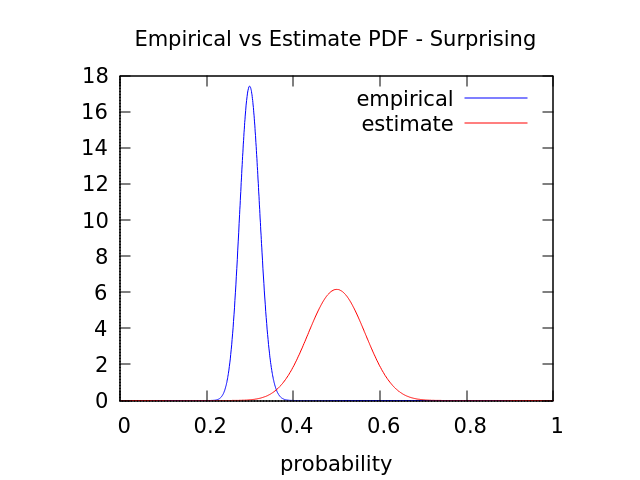
\includegraphics[scale=0.85]{images/surprising.png}}
    \only<2>{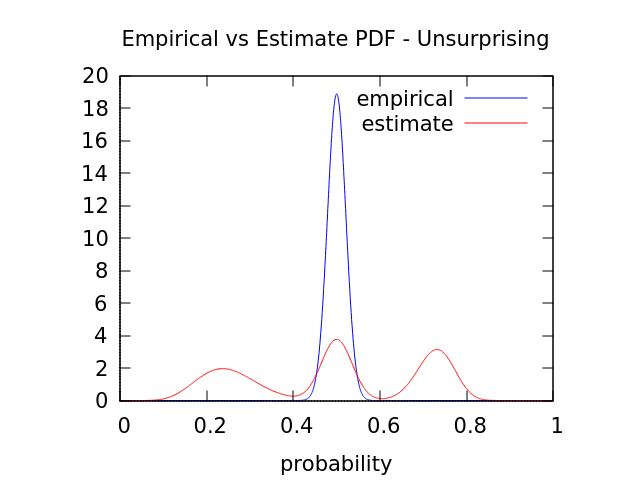
\includegraphics[scale=0.85]{images/unsurprising.png}}
  \end{center}

\end{frame}

\begin{frame}
  \frametitle{Mining Surprising Patterns as Reasoning}

%%%%%%%%%%%%
%% Speech %%
%%%%%%%%%%%%
  
%% OK, so let me run you through that. The surprisingness is defined
%% as the distance between the empirical distribution and the estimate
%% distribution, here the distance is the Jensen-Shannon distance, so
%% to calculate it you need to infer the empirical distribution, this
%% is easy you just run the pattern over the dataset and counts how
%% many time its true relative to the total size of the dataset. The
%% question is how do you infer the estimate, well the answer is
%% anything, maybe something simple, maybe something very complicated
%% that approximates some type of Solomonoff induction. For now, as
%% currently implemented, we just have one hardwired rule, called IS,
%% which stands for Independence Based Surprisingness Estimate,
%% meaning basically that if the pattern is built up as the
%% conjunction of sub-components we assume these components to be
%% independent. Pretty basic.

%% What we would want though is to have any rule of probability theory
%% and logic allowed, except of course DE, the rule for inferring the
%% empirical distribution, and also to be able to use any background
%% knowledge that may relate to that pattern. If we do that, then we
%% can see that the empirical distributions of other patterns
%% previously considered for surprisingness evaluation can be used,
%% since their empirical distribution is necessary to established
%% their surprisingness, and thus will be part of the knowledge based,
%% therefor could be subsequently used. So for instance, let say we
%% want to infer the surprisingness of a pattern involving white cats,
%% and we already have established the surprisingness of an
%% abstraction of it, say the same pattern over cats in general, as
%% opposed to just white cats, and let say such abstraction is very
%% surprising, we obviously already have its empirical distribution,
%% and this could be combined with other rules to obtain a possibly
%% much better estimate of its specialization, thus decreasing this
%% surprisingness, than it would have been obtained from say an
%% independence based type rule that might have given the high
%% surprisingness over the abstraction, and that would have given the
%% same high surprisingness over the white cat specialization. So we
%% can see that such approach naturally leads to a dynamic measure of
%% surprisingness.

%%%%%%%%%%%%%
%% ~Speech %%
%%%%%%%%%%%%%
  
  \only<1>{
  {\small
  \begin{prooftree}
  \AxiomC{$S \leq \texttt{support}(P, \mathcal{D})$}

  \AxiomC{$P$}
  \AxiomC{$\mathcal{D}$}
  \RightLabel{(DE)}
  \BinaryInfC{$\texttt{emp}(P,\mathcal{D})$}

  \AxiomC{\alert{?}}
  \UnaryInfC{$\texttt{est}(P,\mathcal{D})$}

  \RightLabel{(JSD)}
  \BinaryInfC{$\texttt{jsd}(P,\mathcal{D}))$}

  \RightLabel{(S)}
  \BinaryInfC{$\texttt{surprising}(P, \mathcal{D}, \texttt{jsd}(P,\mathcal{D}))$}
  \end{prooftree}
  }
  }

  \only<2>{
  {\small
  \begin{prooftree}
  \AxiomC{$S \leq \texttt{support}(P, \mathcal{D})$}

  \AxiomC{$P$}
  \AxiomC{$\mathcal{D}$}
  \RightLabel{(DE)}
  \BinaryInfC{$\texttt{emp}(P,\mathcal{D})$}

  \AxiomC{\alert{$P$}}
  \AxiomC{\alert{$\mathcal{D}$}}
  \RightLabel{\alert{(IS)}}
  \BinaryInfC{$\texttt{est}(P,\mathcal{D})$}

  \RightLabel{(JSD)}
  \BinaryInfC{$\texttt{jsd}(P,\mathcal{D}))$}

  \RightLabel{(S)}
  \BinaryInfC{$\texttt{surprising}(P, \mathcal{D}, \texttt{jsd}(P,\mathcal{D}))$}
  \end{prooftree}
  }
  }

  \only<3>{
  {\small
  \begin{prooftree}
  \AxiomC{$S \leq \texttt{support}(P, \mathcal{D})$}

  \AxiomC{$P$}
  \AxiomC{$\mathcal{D}$}
  \RightLabel{(DE)}
  \BinaryInfC{$\texttt{emp}(P,\mathcal{D})$}

  \AxiomC{\alert{$\vdots$}}
  \AxiomC{\alert{$\vdots$}}
  \BinaryInfC{\alert{$\vdots$}}
  \AxiomC{\alert{$\vdots$}}
  \BinaryInfC{$\texttt{est}(P,\mathcal{D})$}

  \RightLabel{(JSD)}
  \BinaryInfC{$\texttt{jsd}(P,\mathcal{D}))$}

  \RightLabel{(S)}
  \BinaryInfC{$\texttt{surprising}(P, \mathcal{D}, \texttt{jsd}(P,\mathcal{D}))$}
  \end{prooftree}
  }
  }

  \only<4->{
  {\footnotesize
  \begin{prooftree}
  \AxiomC{$S \leq \texttt{support}(P, \mathcal{D})$}

  \AxiomC{$P$}
  \AxiomC{$\mathcal{D}$}
  \RightLabel{(DE)}
  \BinaryInfC{$\texttt{emp}(P,\mathcal{D})$}

  \AxiomC{\alert{$\texttt{emp}(Q,\mathcal{D})$}}
  \UnaryInfC{\alert{$\vdots$}}
  \AxiomC{\alert{$\vdots$}}
  \BinaryInfC{\alert{$\vdots$}}
  \AxiomC{\alert{$\vdots$}}
  \BinaryInfC{$\texttt{est}(P,\mathcal{D})$}

  \RightLabel{(JSD)}
  \BinaryInfC{$\texttt{jsd}(P,\mathcal{D}))$}

  \RightLabel{(S)}
  \BinaryInfC{$\texttt{surprising}(P, \mathcal{D}, \texttt{jsd}(P,\mathcal{D}))$}
  \end{prooftree}
  }
  }

  \visible<5>{\textcolor{white}{\noindent\makebox[\linewidth]{\rule{10cm}{0.4pt}}}}
  
  \visible<5>{\begin{center}\alert{Dynamic Surprisingness!}\end{center}}
  
\end{frame}

\begin{frame}
  \frametitle{Examples}

%%%%%%%%%%%%
%% Speech %%
%%%%%%%%%%%%

%% TODO

%% So I've done is run our pattern miner over sub-domains of the SUMO
%% ontology, well I did try on the whole SUMO knowledge base but the
%% patterns were too abstract, keep in mind that SUMO is an upper
%% ontology so it deals in priority with the most abstract layer of
%% knowledge, but when I focused on sub-domains instead, I did find
%% interesting results. I'm gonna present a small selection of that
%% and we'll draw some conclusions from there.

%%%%%%%%%%%%%%%
%% ~Speech   %%
%%%%%%%%%%%%%%%

  SUMO: \emph{Suggested Upper Merged Ontology}
  \begin{itemize}
  \item 25K terms
  \item 80K axioms
  \item Covers many domains
    \begin{itemize}
    \item Economy
    \item Finance
    \item Food
    \item Sports
    \item Music
    \item $\dots$
    \end{itemize}
  \item Open Source
  \end{itemize}
\end{frame}

\begin{frame}[fragile]
  \frametitle{Domain: Geography}

{\tiny \begin{semiverbatim}
(EvaluationLink (stv \textcolor{red}{0.98404255} 1)
   (PredicateNode "isurp")
   (ListLink
      (LambdaLink
         (VariableNode "$X")
         (PresentLink
            \textcolor{blue}{(InheritanceLink
               (VariableNode "$X")
               (ConceptNode "SaltWaterArea")
            )
            (InheritanceLink
               (VariableNode "$X")
               (ConceptNode "MaritimeClaimArea")
            )}
         )
      )
      (ConceptNode "sumo")
   )
)
\end{semiverbatim}}

\end{frame}

\begin{frame}[fragile]
  \frametitle{Domain: CountriesAndRegions}

{\tiny \begin{semiverbatim}
(EvaluationLink (stv \textcolor{red}{0.99387284} 1)
   (PredicateNode "nisurp")
   (ListLink
      (LambdaLink
         (VariableList
            (VariableNode "$X")
            (VariableNode "$Y")
         )
         (PresentLink
            \textcolor{blue}{(EvaluationLink
               (PredicateNode "geographicSubregion")
               (ListLink
                  (VariableNode "$X")
                  (ConceptNode "WesternEurope")
               )
            )
            (EvaluationLink
               (PredicateNode "dependentGeopoliticalArea")
               (ListLink
                  (VariableNode "$Y")
                  (VariableNode "$X")
               )
            )}
         )
      )
      (ConceptNode "sumo")
   )
)
\end{semiverbatim}}

\end{frame}

\begin{frame}[fragile]
  \frametitle{Domain: CountriesAndRegions}

%% OK, this is one is interesting, it's very similar to the previous
%% one, it says that European nations tend to be dependent
%% geopolitical areas, so it probably shows the current limit of the
%% system, it's pretty much the previous pattern about Europe instead
%% of Western Europe, and so it probably shouldn't appear as
%% surprising as it does here.

%% TODO: check the instances  

{\tiny \begin{semiverbatim}
(EvaluationLink (stv \textcolor{red}{0.98713296} 1)
   (PredicateNode "nisurp")
   (ListLink
      (LambdaLink
         (VariableList
            (VariableNode "$X")
            (VariableNode "$Y")
         )
         (PresentLink
            \textcolor{blue}{(MemberLink
               (VariableNode "$X")
               (ConceptNode "EuropeanNation")
            )
            (EvaluationLink
               (PredicateNode "dependentGeopoliticalArea")
               (ListLink
                  (VariableNode "$Y")
                  (VariableNode "$X")
               )
            )}
         )
      )
      (ConceptNode "sumo")
   )
)
\end{semiverbatim}}

\end{frame}

\begin{frame}[fragile]
  \frametitle{Domain: CountriesAndRegions}

{\tiny \begin{semiverbatim}
(EvaluationLink (stv \textcolor{red}{0.98350379} 1)
   (PredicateNode "nisurp")
   (ListLink
      (LambdaLink
         (VariableNode "$X")
         (PresentLink
            \textcolor{blue}{(EvaluationLink
               (PredicateNode "meetsSpatially")
               (ListLink
                  (VariableNode "$X")
                  (ConceptNode "NorthAtlanticOcean")
               )
            )
            (MemberLink
               (VariableNode "$X")
               (ConceptNode "AmericanState")
            )}
         )
      )
      (ConceptNode "sumo")
   )
)
\end{semiverbatim}}

\end{frame}

\begin{frame}[fragile]
  \frametitle{Domain: Economy}

{\tiny \begin{semiverbatim}
(EvaluationLink (stv \textcolor{red}{0.97436702} 1)
   (PredicateNode "nisurp")
   (ListLink
      (LambdaLink
         (VariableNode "$X")
         (PresentLink
            \textcolor{blue}{(EvaluationLink
               (PredicateNode "economyType")
               (ListLink
                  (VariableNode "$X")
                  (ConceptNode "AdvancedEconomy")
               )
            )
            (EvaluationLink
               (PredicateNode "economyType")
               (ListLink
                  (VariableNode "$X")
                  (ConceptNode "DevelopedCountry")
               )
            )}
         )
      )
      (ConceptNode "sumo")
   )
)
\end{semiverbatim}}

\end{frame}

\begin{frame}[fragile]
  \frametitle{Domain: Government}

{\tiny \begin{semiverbatim}
(EvaluationLink (stv \textcolor{red}{0.98293616} 1)
   (PredicateNode "nisurp")
   (ListLink
      (LambdaLink
         (VariableNode "$X")
         (PresentLink
            \textcolor{blue}{(EvaluationLink
               (PredicateNode "organizationalObjective")
               (ListLink
                  (VariableNode "$X")
                  (ConceptNode "SocialDevelopment")
               )
            )
            (EvaluationLink
               (PredicateNode "organizationalObjective")
               (ListLink
                  (VariableNode "$X")
                  (ConceptNode "EconomicDevelopment")
               )
            )}
         )
      )
      (ConceptNode "sumo")
   )
)
\end{semiverbatim}}

\end{frame}

\begin{frame}[fragile]
  \frametitle{Examples}

%% This is a small excerpt, there are hundreds more patterns that can
%% be found in 

%% Some are difficult to understand, some are easy to understand, what
%% is interesting is that, often the ones that are understandable tend
%% to be unsurprising, because as humans we're able to utilize our
%% background knowledge to come up with good estimates, better than
%% what our current system can come up with, which demonstrates well
%% the limit of our current system, and one that we hope to overcome
%% by replacing our adhoc estimates with broader reasoning
%% capabilities as to take advantage of background knowledge and
%% dynamic surprisingness.

\end{frame}

\end{document}
